\documentclass[11pt]{article}
\usepackage[margin=0.9in]{geometry}
\usepackage{graphicx,booktabs,amsmath,xcolor,float,hyperref,algorithm,algpseudocode}
\usepackage{mathptmx} % Times New Roman-compatible text and mathematics
\hypersetup{colorlinks=true,linkcolor=blue,urlcolor=blue}
\newcommand{\method}{\textsc{CourtFlow-GS }}
\newcommand{\pro}{\textcolor{red}{[measure on RTX PRO 6000]}}
\title{\method: Online Multi-View Dynamic Gaussian Reconstruction with Fused MLS Tracking}
\author{Shangar Muhunthan}
\date{\today}
\begin{document}
\maketitle

\begin{abstract}
\method turns synchronized videos from cameras around a basketball court into a 3D scene that can
be viewed from a new camera angle. It first builds one clean, static ``starting scene'' from frame
0. It then follows each player through the video by moving small sets of control points, and
occasionally improves visual detail. The result is a 300-frame 3D reconstruction, novel-view
videos, and a saved Gaussian model that can be rendered later without retraining.
\end{abstract}

\section{Problem and data}
The data contains 36 synchronized 4K cameras placed in a ring around the court. Their positions,
orientations, and lenses have already been calibrated, so the system knows exactly where every
camera is. We train with every third camera (views $0,3,\ldots,33$) and keep the remaining 24
cameras aside for an honest test from viewpoints the model did not see during training. The camera
calibration is fixed throughout the method.

The input adapter reads \texttt{cameras/view\_XXX.mp4} together with
\texttt{calibration/cameras.txt} and \texttt{images.txt}. It creates an undistorted,
half-resolution working copy for training. This preserves the camera geometry while making the
many repeated training renders practical on the RTX 3080.

\section{Methodology}
Before doing anything else, every image is undistorted. This removes lens bending, so a straight
camera ray in the mathematics corresponds to a straight ray in the image. In the notation used
later, camera $c$ is $P_c=K_c[R_c\mid t_c]$, with world-to-camera conversion $x_c=R_cx+t_c$.
Readers do not need this equation to follow the method: it only says that the known calibration
projects a 3D point into each image. Camera poses, lens parameters, and per-camera brightness
corrections are kept fixed.

\subsection{Frame-0 Reconstruction}
\paragraph{Masks and 3D identities:}
Photometric reconstruction alone is too ambiguous for the moving players. Each player occupies a
small portion of a frame, shares colour and texture with teammates, and is frequently overlapped
by another player or various structures / elements in the scene. 
Foreground masks tell the system both ``which pixels belong to this person for geometry matching''
and ``where this person is allowed to appear when rendered.''
This prevents background splats from being absorbed into players and prevents players from
growing fuzzy opaque halos onto the court. It also tells the optimizer which
Gaussian/control-point group should explain each pixel.  This prevents a global reconstruction
from improving RGB error by assigning one player's appearance or motion to another player or to
the background.

Simply running a detector in each camera is not enough: ``person 4'' in one image has no reason to
be the same physical person as ``person 4'' in another. We first tried matching 2D mask centres
and colours between cameras. With cameras about $30^\circ$ apart, that split 68 masks into 60
supposed people. Full-frame MASt3R matching was also too coarse for small players and made
unreliable star-shaped rays. Instead, CourtFlow-GS establishes identity \emph{in 3D first}.

Faster R-CNN proposes person boxes (score $\geq0.5$), and SAM2 turns each box into a precise
foreground mask. We use agreement between those masks to make rough 3D blobs, where each blob is
a likely physical player. We project each blob back into every camera and match it to the local
SAM2 mask. When a mask is missing, the projected blob tells SAM2 where to look again. In this way,
noisy per-camera masks become one consistent player ID across the ring.

Concretely, we cover the court with a 2.4 m-high box that extends 1 m beyond the court lines, and
divide it into small cubes called voxels. A voxel is kept only if enough cameras see it inside a
person mask: at least $\max(4,n_{\mathrm{visible}}-2)$ cameras. Put simply, several cameras must
agree, but up to two are allowed to disagree because a player can be hidden. We discard blobs that
are too small, too short, or floating above the floor. A blob wide enough to contain two people is
split on the court floor.

For a missing camera mask, we accept the new SAM2 result only if its colour is similar to that same
3D player in the other cameras. If it still looks wrong, we mark that player as \emph{unknown} in
that camera, not as background. This is important: a hidden or missed player should not teach the
model that the court is visible there. Finally, if two accepted masks overlap, the closer player
owns the pixel. The result is one label image $L_c$ per camera in which every pixel is either
background or exactly one player. Later, this lets every player have separate Gaussian splats and
separate motion controls.

\paragraph{Occlusion-aware visual hull.}
A visual hull is a rough 3D body made by intersecting the player silhouettes from several cameras.
The usual rule says to remove a voxel if even one camera does not see the player there. That works
for a clean object on a turntable, but fails in basketball: another player, the hoop support, or
padding can hide a real arm, leg, or head. We saw those missing body parts with a strict hull.

The opposite rule, forgiving any missing view---was also bad. One allowed miss made player hulls
about $2.5\times$ too large. Our compromise asks one simple question: \emph{is there measured
evidence that something closer to this camera was blocking the player?} We forgive a missing pixel
only when the answer is yes. This is what ``occlusion-aware'' means here.

For each player, we test a fine 1 cm grid inside the rough 3D blob, with a small margin. Camera
$c$ votes against a candidate voxel $x$ only when the voxel is visible in that camera, the player
has a trusted label there, the projected pixel is not labelled as that player, and nothing nearer
explains why. A nearer explanation can be another labelled player or a measured background surface
(such as the hoop support) at least 30 cm in front. The background depth map $D_c$ comes from
reliable full-frame MASt3R background points that agree in at least two additional cameras. We
retain the nearest depth at each image location and ignore floor points within 0.5 m of the court.

We keep $x$ when at least two cameras see it as the player and no camera has an \emph{unexplained}
reason to reject it. Voxels below the floor are then removed. A camera where the player is unknown
casts no vote. Thus the method does not keep geometry merely because occlusion might be possible;
it keeps it only when a nearer player or surface actually supports that explanation.

\paragraph{Masked crop geometry and Gaussian seeds.}
Feature matching across a full image works for the court, but a distant player may occupy only
about $6\times25$ pixels once MASt3R shrinks the whole frame to 512 pixels. Our full-frame player
matches made a radial ``star'' of unreliable 3D rays. The masks solve this by giving the player
the full matching resolution: for nearby camera pairs, we crop a padded square around the same 3D
player and resize that crop to $512\times512$. MASt3R searches only inside the source player mask.

After mapping matches back into the original camera images, we retain only confident matches that
are in front of the cameras, reproject accurately, use cameras far enough apart for useful depth,
lie inside a slightly expanded player hull, and agree with at least one more labelled camera. This
removes the court and background rays that slipped through earlier mask-only tests.

The retained matches are accurate surface seeds. Hull voxels fill only textureless gaps more than
two hull voxels away from a seed. We colour points only from cameras that agree with the label and
can actually see the point, remove outliers, merge nearby player points at 5 mm and background
points at 10 cm, and turn the result into oriented, elongated Gaussian splats. Each Gaussian stores
position, shape, opacity, and simple view-dependent colour (degree-1 spherical harmonics).
Players train for 7000 iterations (four cameras per step) and background for 10000 (two cameras
per step), using
\[
\mathcal L_{\rm image}=\|I-\hat I\|_1+0.2\,\mathrm{D\mbox{-}SSIM}
+0.1\mathcal L_{\rm alpha}+0.05\mathcal L_{\rm depth}.
\]
This loss asks the rendered image to match the real image, its structure, its silhouette, and its
initial depth. The depth term fades out halfway through training, after it has helped establish the
coarse shape. Starting at iteration 500, we add detail where needed every 100 iterations until
halfway through training. We remove nearly transparent splats and splats that land outside an
expanded player mask in two cameras.

\subsection{Group-aware control-point MLS}
\paragraph{Why use separate control groups?}
After frame 0, the task is to move the same Gaussian splats as players move. Rather than moving
millions of splats independently, we place a much smaller set of control points on each player.
Moving a control point moves nearby splats smoothly. This is called moving-least-squares (MLS)
deformation.

A single global control graph is reasonable for one connected object, but unsafe in a crowded game.
Controls on two nearby players can otherwise explain the same image error, causing one player to
pull another player's splats or the background. CourtFlow-GS treats every identity as a separate
motion group. This keeps the useful smooth motion of MLS while forbidding cross-player influence.

Every dynamic Gaussian belongs to exactly one person; the ball, when enabled, is another group,
and background is group 0. We choose controls spread evenly over each object: 1024 per person,
16 for the ball, and 1000 for background. Each Gaussian is permanently connected to its eight
nearest controls from the \emph{same} group. Closer controls get more influence through the fixed
radial weights
\[
w_{ij}=\frac{\exp(-\|x_i-p_j\|^2/(2\sigma_j^2))}
{\sum_{\ell=1}^{8}\exp(-\|x_i-p_\ell\|^2/(2\sigma_\ell^2))},
\]
where $\sigma_j$ is the average distance to control $j$'s three nearest controls. The six nearest
same-group controls form the shape-preserving ARAP graph. In plain terms, a player's splats follow
that player's nearby controls, never a teammate's or the court's.

\paragraph{Why shared translation plus local motion?}
Trying to move every control independently made weakly observed controls lag or drift. By frame 10
that version reached 0.60 mask overlap (IoU), compared with 0.71 when each player first gets one
shared translation and then small local offsets. The shared translation handles running across the
court; the local offsets handle arms, legs, and other articulation. A rigid local MLS transform
and the ARAP shape loss keep neighbouring splats from stretching apart.

At frame $f$, controls begin from the previous frame's velocity. We optimize one shared translation
$T_k$ per moving group and small local offsets $\delta_j$ for 50 Adam iterations, using four
cameras per iteration. Their learning rates are 0.020 m and 0.003 m. Let
$t_j=T_{g(j)}+\delta_j$ and $p'_j=p_j+t_j$. For Gaussian $i$, the fixed weights above blend nearby
original controls $p_j$ and moved controls $p'_j$ to form a best local rotation $R_i$:
\[
 \bar p_i=\sum_jw_{ij}p_j,\quad \bar q_i=\sum_jw_{ij}p'_j,\quad
 M_i=\sum_jw_{ij}(p_j-\bar p_i)(p'_j-\bar q_i)^T.
\]
With $M_i=USV^T$, set $R_i=VU^T$, flipping the last column of $V$ if $\det(VU^T)<0$. The final
Gaussian position is $x'_i=R_i(x_i-\bar p_i)+\bar q_i$; its orientation and simple colour direction
are rotated too. A fused CUDA operation performs this transform and its backward pass. The reported
run does not separately optimize control rotations.

Every fifth frame, we render where each player is expected, prompt SAM2 with that box and centre,
and assign overlapping pixels to the strongest rendered player. We triangulate the 2D mask centres
from several cameras into a rough 3D player centre. This is a \emph{motion anchor}: it gives the
shared translation a reliable hint about where a player moved, especially after fast motion or
occlusion. If enough cameras see the player, a robust Huber anchor of scale 0.3 m and weight 0.1
is used. Between those frames, no made-up mask or anchor is used. The deformation objective is
\[
\mathcal L=\mathcal L_{\rm image}+0.3\mathcal L_{\rm BCE}^{\rm instance}
+\mathcal L_{\rm ARAP}+0.01\mathcal L_{\rm accel}+\mathcal L_{\rm anchor},
\]
Here the image term matches appearance, BCE matches each player's rendered mask, ARAP preserves
local shape, acceleration discourages sudden jitter, and the anchor discourages global drift.
Background controls stay frozen while the moving splats are rendered over a cached background.

\begin{figure}[H]
\centering
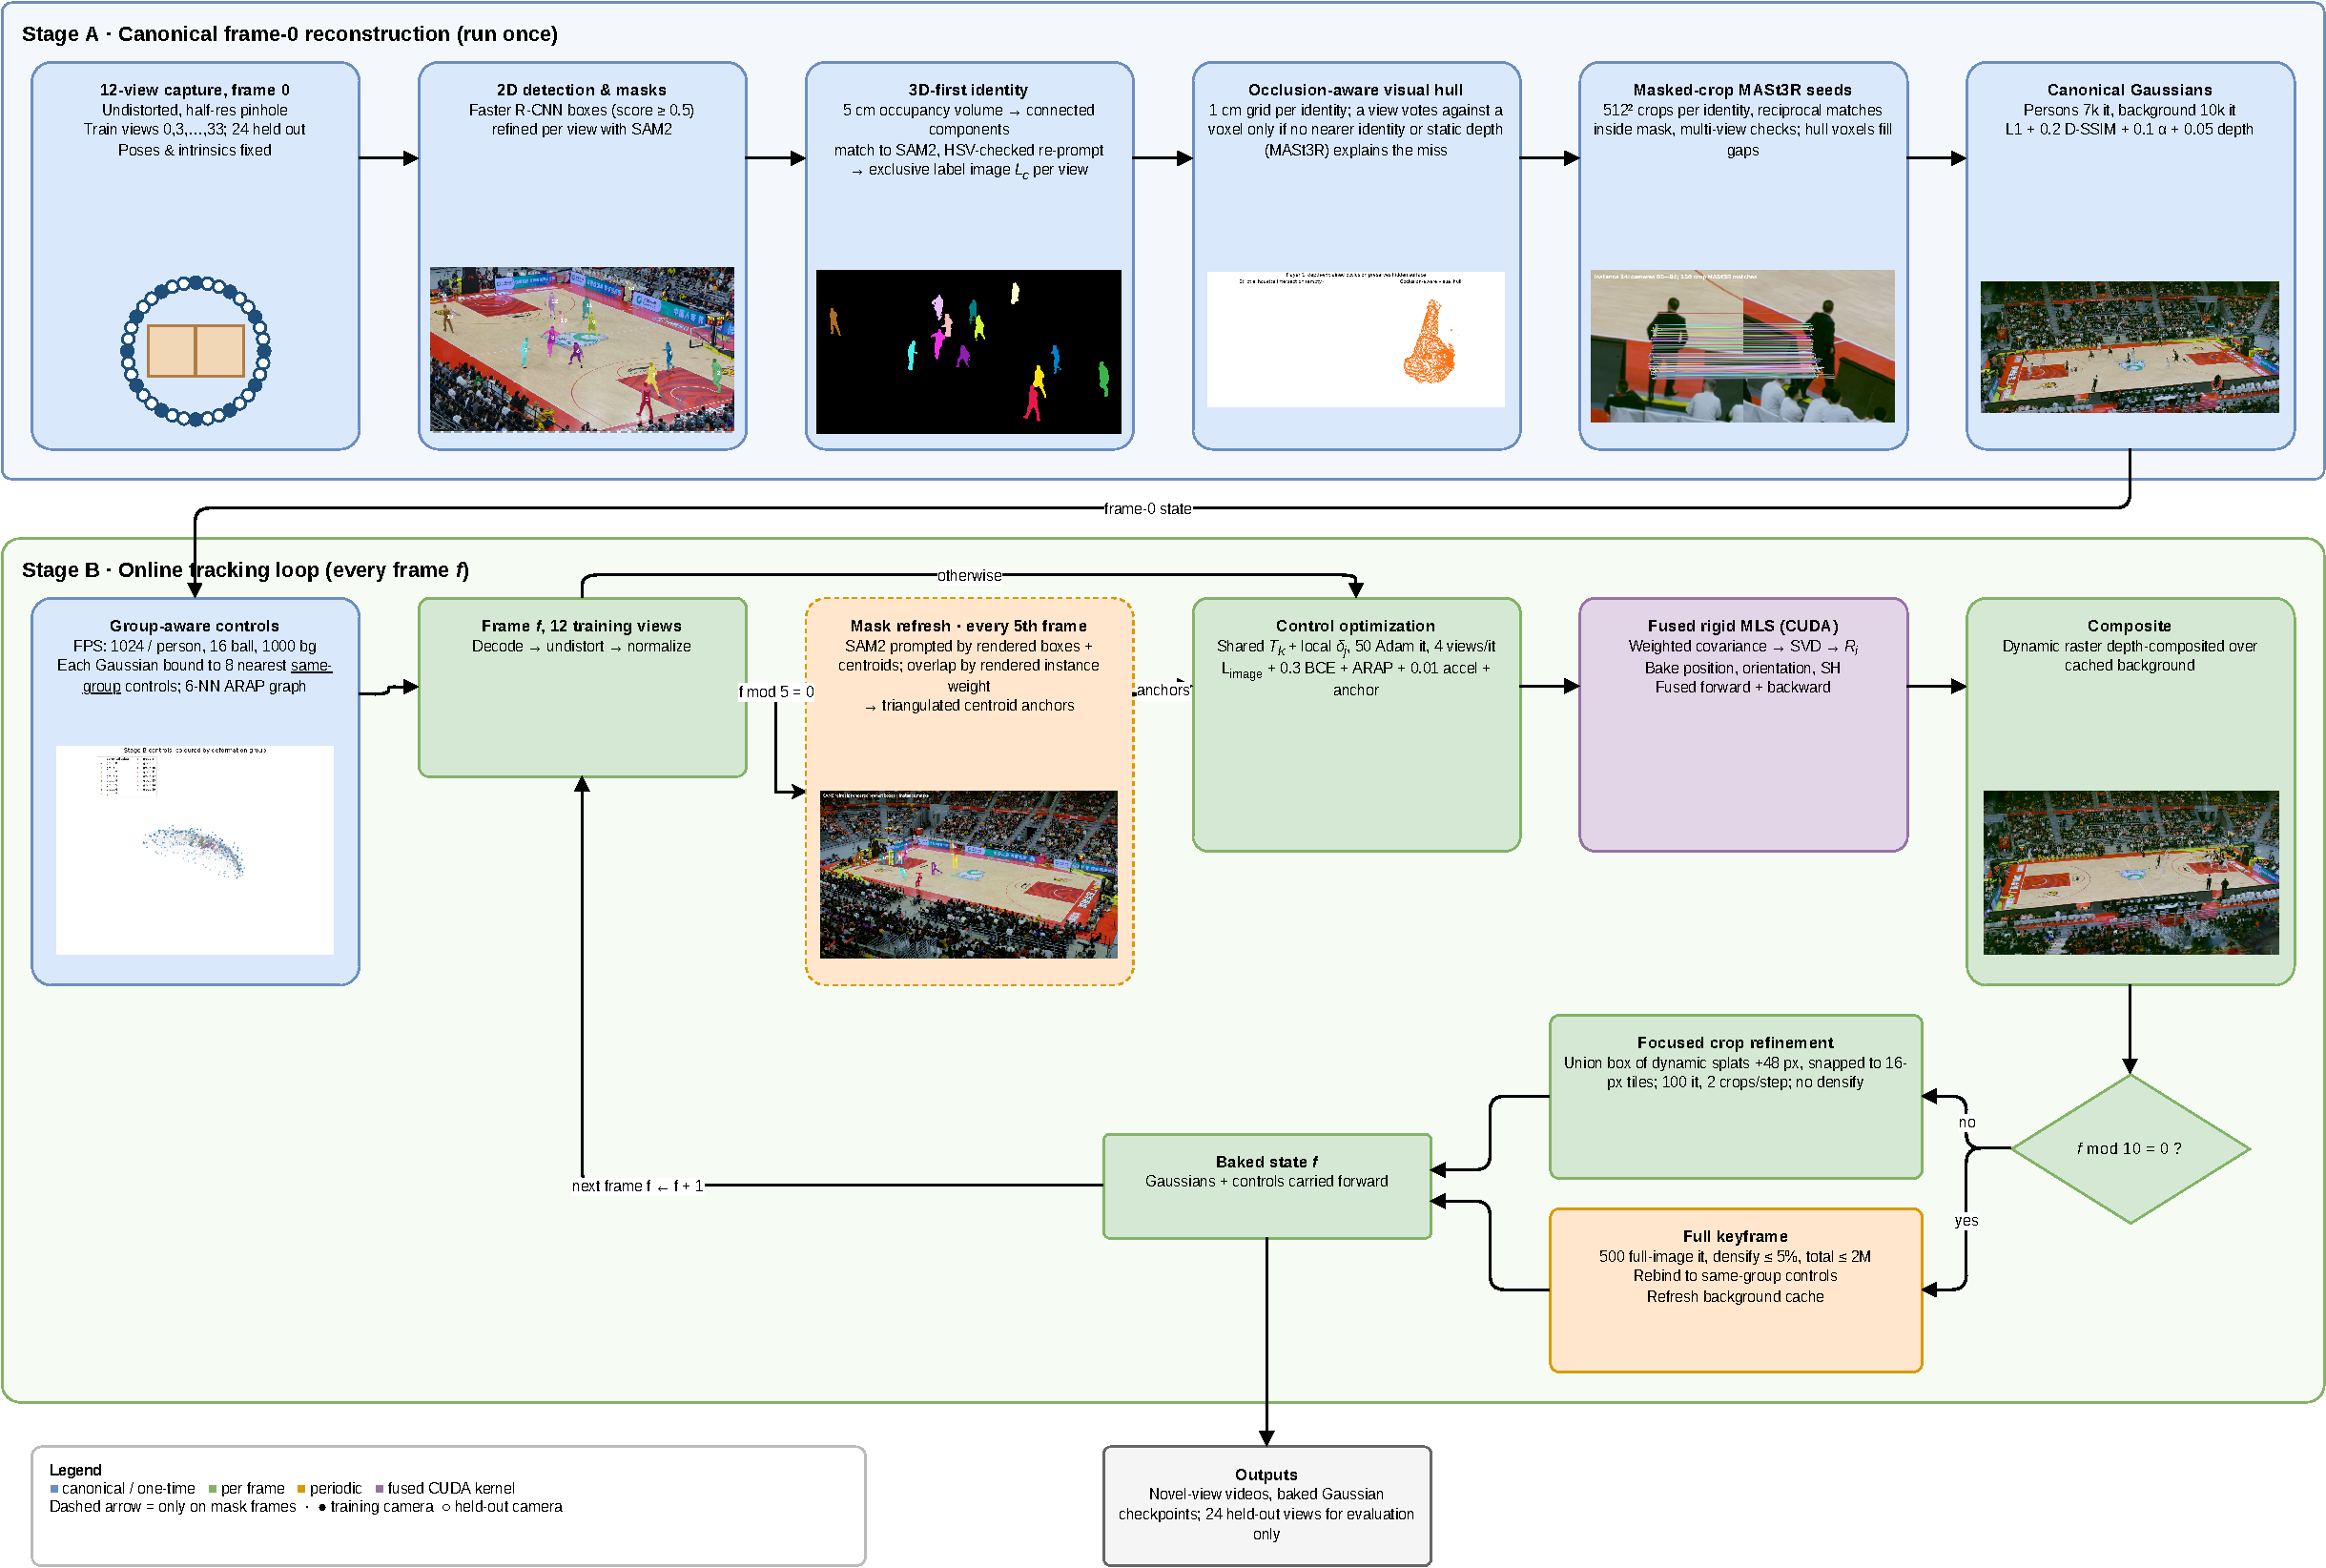
\includegraphics[width=\linewidth,height=4.0in,keepaspectratio]{figures/courtflow_gs_pipeline.pdf}
\caption{CourtFlow-GS pipeline. The editable diagram source is distributed with the report as
\texttt{courtflow\_gs\_pipeline.drawio}.}
\end{figure}

\subsection{Focused refinement}
MLS provides stable, smooth motion, but deliberately does not change a Gaussian's colour, size, or
amount of detail. Updating the full image after every video frame would be wasteful: players cover
less than 1\% of the court image, so most compute would repeatedly optimize the static floor. We
therefore refine only the moving-player crops most frames, and use occasional full-image keyframes
to correct drift and add a limited amount of new detail.

After every deformation, we save (``bake'') the moved Gaussian and control state for that frame.
On a normal frame, all moving splats are projected into each training camera and surrounded by one
box with 48 pixels of padding. The box is aligned to the rasterizer's 16-pixel tiles, and the camera
principal point is shifted so rendering the crop is exactly equivalent to rendering that part of
the full image. We run 100 refinement iterations on two crops per step. No splats are added or
removed here, so their control bindings stay stable.

Every tenth frame is a keyframe. It instead runs 500 full-image iterations, can add splats from
iteration 50 every 50 iterations until 60\% of the schedule, and limits growth to 5\% per keyframe.
It then reconnects each Gaussian to its eight nearest same-group controls and refreshes the cached
background. Held-out cameras are never included in any training loss.

\subsection{Pseudocode}
Algorithm~\ref{alg:courtflow} summarizes the whole process. The helper names are intentionally
literal: first build the frame-0 scene, then for each video frame estimate motion, bake that motion,
and improve either player crops or a periodic full keyframe.
\begin{algorithm}[H]
\caption{CourtFlow-GS online reconstruction}\label{alg:courtflow}
\begin{algorithmic}[1]
\Require Frame-0 images, synchronized training videos, fixed calibration
\State $(\mathit{state},\mathit{controls}) \gets \textsc{BuildCanonicalScene}(\mathit{frame}_0,\mathit{calibration})$
\For{each $f$ in the video sequence}
  \State $\mathit{images} \gets \textsc{DecodeUndistortNormalize}(\mathit{trainingVideos},f)$
  \If{$f \bmod 5 = 0$}
    \State $\mathit{masks} \gets \textsc{RepairMultiViewSAM2Identities}(\mathit{images},\mathit{state.dynamic})$
    \State $\mathit{anchors} \gets \textsc{TriangulateMaskCentroids}(\mathit{masks})$
  \Else
    \State $\mathit{masks},\mathit{anchors} \gets \emptyset,\emptyset$
  \EndIf
  \State $\mathit{offsets} \gets \textsc{OptimizeControls}(L_1{+}\mathrm{D\text{-}SSIM},\mathit{masks},\mathit{anchors},\mathrm{ARAP})$
  \State $\mathit{state} \gets \textsc{BakeFusedRigidMLS}(\mathit{state},\mathit{controls},\mathit{offsets})$
  \If{$f \bmod 10 \ne 0$}
    \State $\mathit{state} \gets \textsc{RefineDynamicCrops}(\mathit{state},\mathit{images},100)$
  \Else
    \State $\mathit{state} \gets \textsc{RefineFullImages}(\mathit{state},\mathit{images},500)$
    \State $\mathit{controls} \gets \textsc{Rebind}(\mathit{state},\mathit{controls})$; \textsc{CacheBackground}($\mathit{state}$)
  \EndIf
  \State \textsc{SaveDiagnostics}($\mathit{state}$)
\EndFor
\end{algorithmic}
\end{algorithm}

\section{Results}
The final diagnostic reconstructs 300 frames. PSNR measures image similarity in decibels (higher is
better); person PSNR measures it only on player regions; IoU measures how well predicted and true
player masks overlap (1 is perfect). The diagnostic's held-out result is the important generalization
measurement because those cameras were never trained on.
\begin{table}[H]\centering
\caption{Quality summary. Temporal held-out samples coincide with keyframes.}
\begin{tabular}{lrrrr}\toprule
Method & Full PSNR & Person PSNR & Person IoU & Measurement \\\midrule
Global 3DGS baseline & 17.50 & -- & -- & frame-0 held-out \\
Stage A canonical & 19.32 & 18.34 & 0.788 & frame-0 held-out \\
Stage B v1 & 18.29 & 15.00 & 0.70$\rightarrow$0.30 & keyframe held-out mean \\
Stage B v2 (old) & 18.87 & 19.62 & 0.71$\rightarrow$0.39 & keyframe held-out mean \\
Focused refinement, frames 1--20 & 22.42 & 26.76 & 0.746 & training-view mean \\
Final 300-frame diagnostic & 20.07 & 22.44 & -- & held-out mean \\\bottomrule
\end{tabular}\end{table}

\begin{figure}[H]\centering
\begin{minipage}[b]{.32\linewidth}\centering
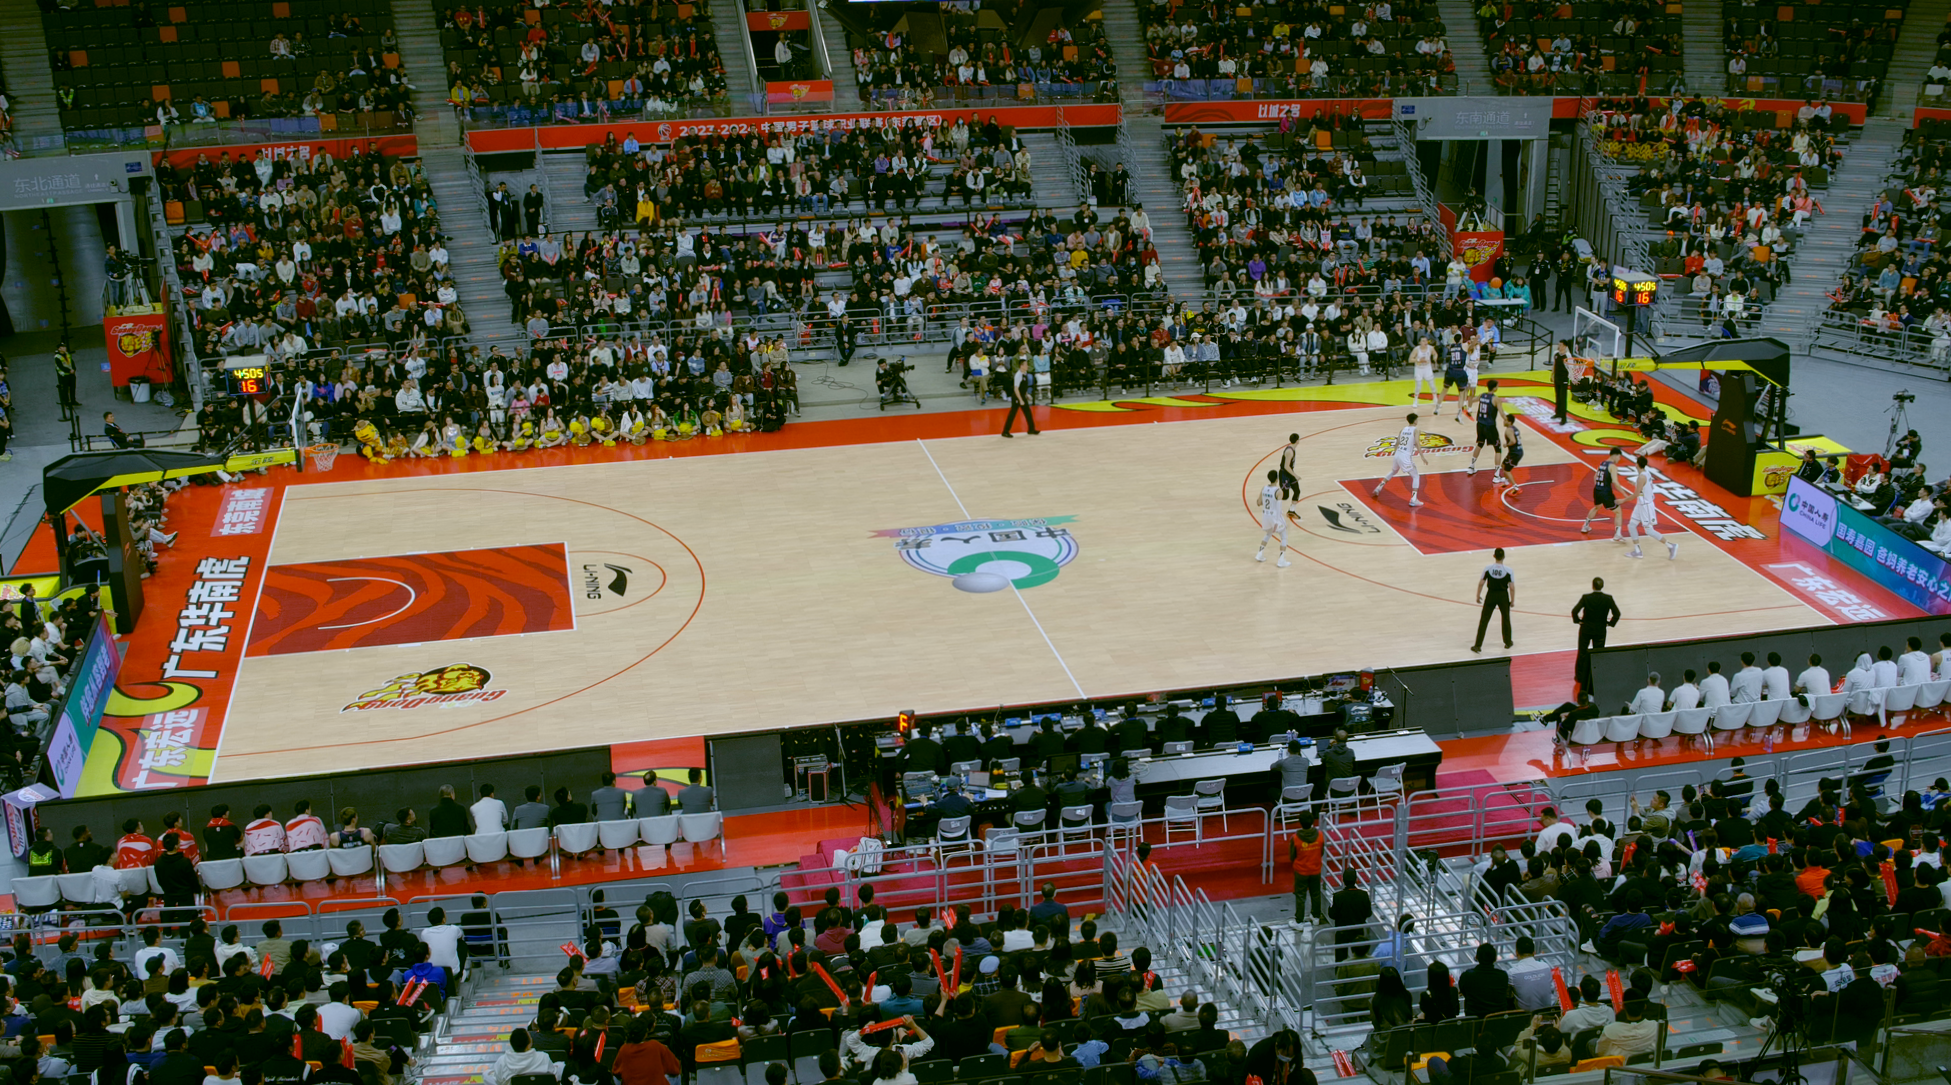
\includegraphics[width=\linewidth]{figures/view13_gt_f200.png}\\\small Ground truth, view 13, frame 200
\end{minipage}\hfill
\begin{minipage}[b]{.32\linewidth}\centering
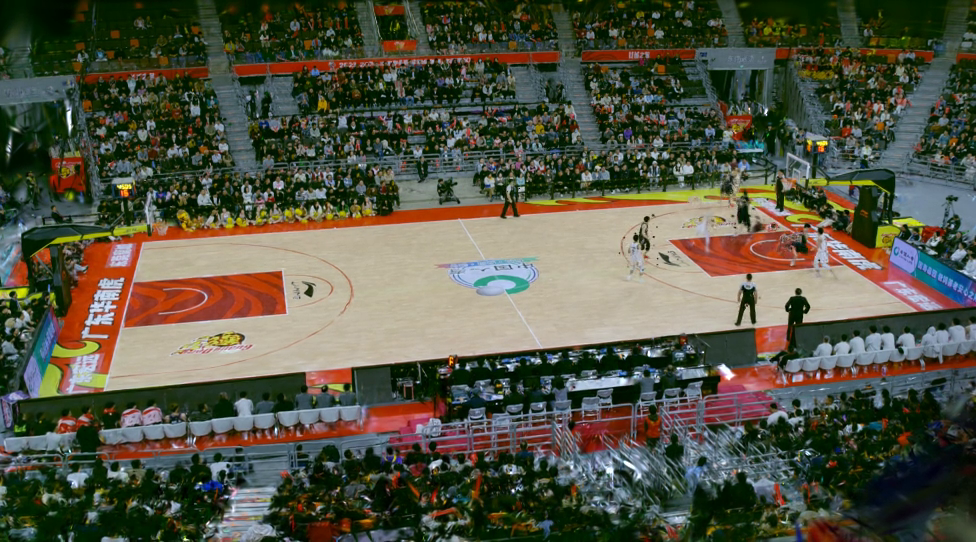
\includegraphics[width=\linewidth]{figures/view13_v2_f200.png}\\\small Earlier Stage B v2
\end{minipage}\hfill
\begin{minipage}[b]{.32\linewidth}\centering
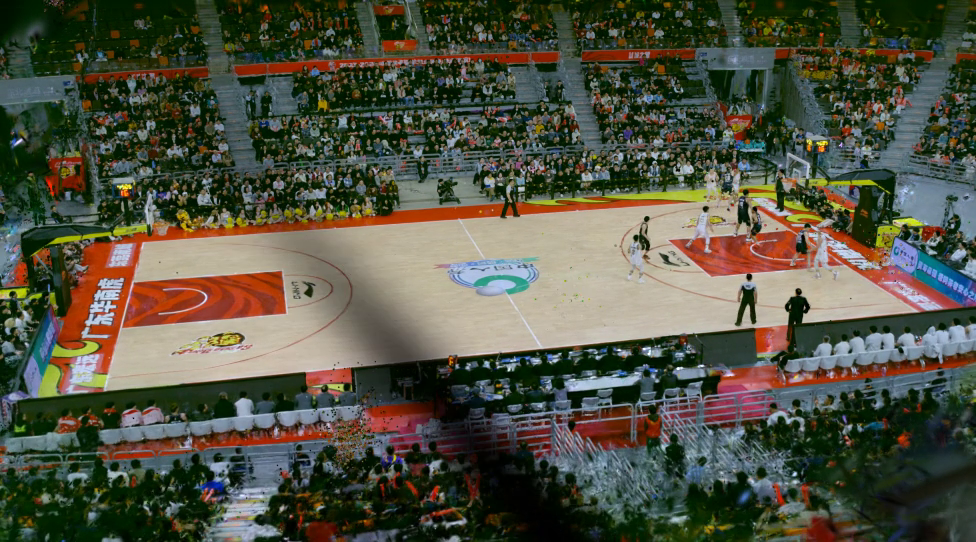
\includegraphics[width=\linewidth]{figures/view13_courtflow_f200.png}\\\small CourtFlow-GS diagnostic
\end{minipage}
\caption{Same-camera comparison at held-out view 13, frame 200. Replace or add comparison rows as desired.}
\end{figure}

\subsection{Why these design choices were selected}
The method was not chosen by adding complexity for its own sake. Table~\ref{tab:choices} records
the practical failures we observed and the smallest change that addressed each one. These are useful
trade-offs: some choices improve quality and speed at the same time by avoiding work on irrelevant
pixels, while others deliberately spend more computation only where player detail needs it.
\begin{table}[H]\centering
\caption{Design choices and the observation behind each one.}\label{tab:choices}
\small\begin{tabular}{p{.31\linewidth}p{.61\linewidth}}\toprule
Choice & Why it was selected \\\midrule
3D-first identities & Matching 2D centres and colours independently fragmented 68 masks into 60 apparent people. Building rough 3D components first gives the same player one ID across cameras. \\
Occlusion-aware hull & A strict silhouette intersection removed hidden limbs. Allowing arbitrary misses inflated a hull by about $2.5\times$. Measured nearer depth supplies the middle ground. \\
Masked MASt3R crops & Full-frame descriptors reduce a small player to about $6\times25$ pixels and produced star-shaped rays. Crops spend the fixed descriptor resolution on the player instead of the court. \\
Same-group MLS controls & A global control graph lets nearby teammates pull each other. Fixed same-player control neighbours keep motions separate and also make deformation cheap. \\
Shared translation plus local offsets & Moving every control alone reached 0.60 IoU by frame 10; shared translation plus local articulation reached 0.71 IoU. \\
Crop refinement plus keyframes & Full-image updates mostly optimize static court pixels. Player crops improve moving detail cheaply; full keyframes occasionally correct accumulated error and add splats. \\\bottomrule
\end{tabular}\end{table}

\subsection{Evaluation protocol and deliverables}
The 12 training cameras are never used as novel-view evidence. At every tenth frame and at the final
frame, the tracker renders all 24 held-out cameras and compares them to their synchronized real
images. The current report gives full-frame PSNR and player-region PSNR; player-region IoU checks
whether the rendered player footprint agrees with the independent mask. The final RTX PRO 6000 run
will report the mean and standard deviation over the held-out camera/frame pairs, together with
SSIM and LPIPS, and will include a grid of easy, crowded, and occluded held-out views. This makes
it clear that quality is measured from cameras the model did not optimize against.

The release command produces two animated deliverables during tracking: a held-out camera video
and an orbit video. These renders use the state from each corresponding video frame. This matters
because one baked PLY checkpoint is a snapshot at one instant; repeating the final snapshot would
make a static movie, not an animation. The editable canonical model, controls, and calibration are
kept for re-training or editing. The final source scene is about 150 MB on the RTX 3080; a naive
per-frame PLY bake would be about 42 GB for 300 frames, so a deployable animated package should use
packed, quantized frame chunks rather than text PLY files.

\section{RTX 3080 runtime}
\begin{table}[H]\centering
\caption{Runtime. A frame normally uses MLS, crop refinement, and occasionally the more expensive
keyframe step.}\begin{tabular}{lrr}\toprule
Component & RTX 3080 12 GB & RTX PRO 6000 \\\midrule
MLS deformation/control optimization & 1.95 s/frame & \pro \\
Focused crop refinement & 3.41 s/non-keyframe & \pro \\
500-step full keyframe & 23.16 s/keyframe & \pro \\
Mask refresh, amortized & 0.33 s/frame & \pro \\
End-to-end diagnostic & 7.61 s/frame (0.131 FPS) & \pro \\
GPU SH colour + baked raster, 937$\times$527 & 4.36 ms (229 FPS) & \pro \\\bottomrule
\end{tabular}\end{table}

The fused MLS/SVD calculation is only a small part of tracking time. Rendering and differentiating
through the rasterizer dominate optimization. Once motion is baked, GPU rendering is fast; the
current video exporter is instead limited by copying frames from Python to ffmpeg.

The frame-0 canonical build took 1896 s (31.6 min) on the RTX 3080, including geometry, crops,
fusion, and Gaussian training. The 300-frame diagnostic's measured 7.61 s/frame corresponds to
about 38.1 min for Stage B alone. These are 3080 reference measurements, not extrapolations to the
PRO 6000. The complete 700-frame PRO 6000 run will replace the placeholders above with measured
wall-clock time, peak VRAM, and inference time at stated 1080p and 4K resolutions.

\section{Limitations and next steps}
The main remaining weakness is identity tracking in crowded late-game plays. Independent SAM2 masks
can swap people or disappear. In the previous diagnostic, training IoU falls from 0.789 near the
start to 0.001 at frame 299; held-out person PSNR falls from 23.86 to 20.59 dB. The production
configuration now repairs SAM2 identities in 3D at mask frames and performs conservative keyframe
recovery when a repaired mask shows that a player was lost. The 300-frame repair run tests whether
that change removes the observed failure rather than merely moving it later in the sequence. Other
useful work is a smaller or level-of-detail version of the 2.01M-Gaussian final state, unbiased
inter-keyframe held-out evaluation, and direct GPU-to-NVENC video output.
\end{document}
